\documentclass{article}
\usepackage{graphicx} % Required for inserting images
\graphicspath{ {./images/} }

\title{MS-CS Master Course Note (Non-Credit)}
\author{Mark Zhou}
\date{March 2024}

\usepackage{setspace}
\usepackage{listings}
\usepackage{amssymb}
\usepackage{amsmath}

\begin{document}
\maketitle
\doublespacing

\paragraph{This is my course note on “Essential Linear Algebra for Data Science” provided by Colorado University of Boulder. 
This is a non-credit prep course for an MS-CS degree.}

\newpage
\tableofcontents
\newpage

\section{Linear Systems and Gaussian Elimination}

\subsection{Linear Systems}

\paragraph{In a linear system, we normally have constants and variables. The constants are the coefficients of the variables. The variables are the unknowns.\\
For example, $a_1*x_1 + a_2*x_2 + \cdots + a_n*x_n = b$ is a linear system. For this to work the variables and constants must be linear. 
That is, the variables must be raised to the power of 1.\\
Neither the product of variables nor the square root of them is allowed.\\
The linear system can be represented in matrix form as $Ax = b$.\\
Where A is the matrix of coefficients, x is the vector of variables, and b is the vector of constants.\\
\hfill
For example, the following is a linear system:\\
$2x_1 + 3x_2 = 5$\\
$4x_1 + 5x_2 = 6$\\
This can be represented as:\\
$\begin{bmatrix} 2 & 3 \\ 4 & 5 \end{bmatrix} 
\begin{bmatrix} x_1 \\ x_2 \end{bmatrix} = 
\begin{bmatrix} 5 \\ 6 \end{bmatrix}$\\}

\paragraph{When we have a linear system, we can have three possibilities.\\
1. The system has a unique solution.\\
2. The system has no solution.\\
3. The system has infinite solutions.\\
\hfill
For example, the following system has a unique solution:\\
$2x_1 + 3x_2 = 5$\\
$4x_1 + 5x_2 = 6$\\
This system has a unique solution of $x_1 = 1$ and $x_2 = 1$.\\
\hfill
Second, the following system has no solution:\\
$2x_1 + 3x_2 = 5$\\
$4x_1 + 6x_2 = 6$\\
Which means there's no cross in the coordinate visualization system.\\
\hfill
And the following system has infinite solutions:\\
$2x_1 + 3x_2 = 5$\\
$4x_1 + 6x_2 = 10$\\
Which means they are actually plotting on the same line.\\}

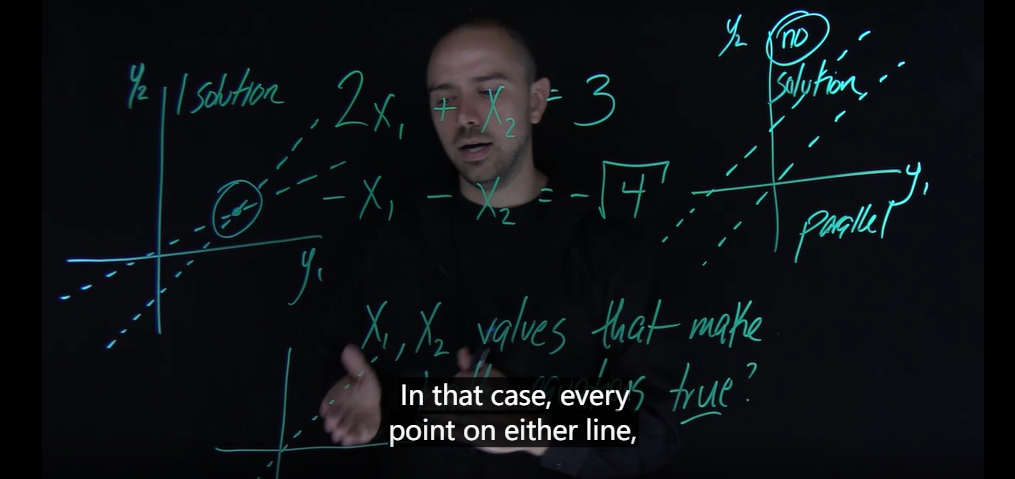
\includegraphics[width=\textwidth]{threesolutions}


\subsection{Matrices and Gaussian Elimination}

\paragraph{As displayed above, we can convert a linear system into a matrix form.\\
The matrix form is $Ax = b$.\\
Where A is the matrix of coefficients, x is the vector of variables, and b is the vector of constants.\\
\hfill
If we extract all the coefficient, a.k.a. the constant values from the matrix, we get the Coefficient Matrix.\\
For example, the following is a linear system:\\
$2x_1 + 3x_2 = 5$\\
$4x_1 + 5x_2 = 6$\\
The Coefficient Matrix can be represented as:\\
$\begin{bmatrix} 2 & 3 \\ 4 & 5 \end{bmatrix}$\\
\hfill
Besides, we can also add the result of the linear system to the matrix, which make a coefficient matrix into an augmented matrix.\\
Here is the augmented matrix of the above linear system:\\
$\begin{bmatrix} 2 & 3 &|& 5 \\ 4 & 5 &|& 6 \end{bmatrix}$\\}





\end{document}